\documentclass[11pt,                                          % Main text font size
a4paper,                                       % Paper size
% Chapters start on odd pages (right)
twoside]{report}                               % Print two-sided, LaTeX 'report' template

% -------------------------------------------------------------
% PACKAGES - Only load if necessary / used
% -------------------------------------------------------------
\usepackage{microtype}                                        % Tweak font spacing for aesthetics
\usepackage{cmbright}                                         % SS font - Comment this line for LaTeX base font
\usepackage[utf8]{inputenc}                                   % Includes letters with accents
\usepackage[T1]{fontenc}                                      % 8-bit encoding with 256 glyphs
\usepackage[colorlinks=true, allcolors=black]{hyperref}       % Hyper-references in PDF (e.g. urlcolor=blue)
\usepackage{fancyhdr}                                         % Headers and footers
\usepackage{subfigure}                                        % Multiple figures environment
\usepackage{amsmath}                                          % Standard maths
\usepackage{amssymb}                                          % Standard maths symbols
\usepackage{graphicx}                                         % Include graphics
\usepackage{booktabs}                                         % Professional tables
\usepackage[english]{babel}                                   % Babel and language definitions
\usepackage[a4paper,                                          % Paper size
top = 35mm,                                       % Top margin
bottom = 30mm,                                    % Bottom margin
left = 35mm,                                      % Left margin
right = 25mm]{geometry}                           % Right margin
\usepackage{nomencl}                                          % Include nomenclature
\usepackage[page,toc,titletoc,title]{appendix}                % Include appendixes
\usepackage{csquotes}                                         % For inline and display quotations
\usepackage{lipsum}                                           % Generate automatic text - Lorem Ipsum
\usepackage{moreverb}                                         % Output for word and character count
\usepackage{tcolorbox}                                        % Coloured boxes
\usepackage{xcolor}                                           % Advanced colours
\usepackage{soul}                                             % Highlight text and other text things
\usepackage{caption}                                          % Manage captions in floats
\usepackage{chemfig,chemformula}                              % Use chemistry formulae
\usepackage{pgfgantt}                                         % Use a Gantt chart
\usepackage{pdflscape}                                        % Landscape pages
\usepackage{cite}                                             % Compressed and sorted lists of citations
\usepackage{listings}                                         % Displayed code
\usepackage{siunitx}                                          % Easy unit 
\usepackage{graphicx}

% -------------------------------------------------------------
% USER VARIABLES AND DEFINITIONS                              % EDIT THIS SECTION
% -------------------------------------------------------------
%\newcommand{}{}
\newcommand{\theTitle}{AR4Learn: Transforming Moroccan Education Through Augmented Reality}            % Thesis title
\newcommand{\runningTitle}{Short thesis title}                % Short title for headers
\newcommand{\theAuthor}{A.U.  \textbf{Thor}}                  % Author name
\newcommand{\theSupervisor}{S.U. Pervisor}                    % Name of supervisor
\newcommand{\mrm}[1]{\mathrm{#1}}
\newcommand{\al}{\alpha}

\definecolor{mygreen}{RGB}{28,130,0}                          % Define your own colours
\definecolor{ocre}{RGB}{45,105,145} 
\definecolor{barblue}{RGB}{153,204,254}                       % Used in Gantt chart
\definecolor{groupblue}{RGB}{51,102,254}                      % Used in Gantt chart
\definecolor{linkred}{RGB}{165,0,33}                          % Used in Gantt chart

%\captionsetup[table]{skip=6pt}                                % Gap between captions and tables
\graphicspath{{Images/}}                                      % Path to folder where pictures are stored
\makenomenclature                                             % Create a nomenclature
\setlength{\nomlabelwidth}{10mm}                              % Set width of nomenclature label
\setlength{\headheight}{14pt}                                 % Minimum hadhight length

% -------------------------------------------------------------
% NOTATION AND ACRONYMS (DEFINITIONS)
% -------------------------------------------------------------
\newcommand{\notitem}[2]{{$#1$} & {~ -- ~ #2}}
\newcommand{\acritem}[2]{{#1} & {~ -- ~ #2}}

% -------------------------------------------------------------
% HEADERS AND FOOTERS
% -------------------------------------------------------------
\fancyhead[LE,RO]{\slshape\nouppercase{\leftmark}}            % Header right-odd and left-even: chapter title
\fancyhead[CE,CO]{}                                           % Header centre-odd and centre-even: empty
\fancyhead[LO,RE]{\slshape\nouppercase{\rightmark}}           % Header left-odd and right even: section title
\fancyfoot[LE,RO]{\thepage}                                   % Footer right-odd and left-even: page number
%\fancyfoot[LE,RE]{\thepage}                                  % Footer right-odd and left-even: page number
%\fancyfoot[R]{\thepage}                                      % Footer right-odd and left-even: page number
\fancyfoot[CE,CO]{}                                           % Footer centre-odd and centre-even: empty
\fancyfoot[LO,RE]{DEVJAM 3.0}                                 % Footer left-odd and right-even: author name
%\fancyfoot[L]{\theAuthor}                                    % Footer left-odd and right-even: author name

% ------------------------------------------------------------------
% DATA PLOTTING AND SETTINGS
% ------------------------------------------------------------------
\usepackage{tikz}
\usepackage{tikz-3dplot}
\usetikzlibrary{calc,backgrounds,matrix}
\usetikzlibrary{shapes,arrows,shapes.multipart}                % For flowcharts, diagrams etc
\usepackage{pgfplots}
\usepackage{pgfplotstable}                                    % Generates table from .csv
\pgfplotsset{compat=newest}
\usetikzlibrary{shapes,positioning,intersections,quotes,fit,patterns}
\usepgfplotslibrary{patchplots}
\pgfplotsset{compat = 1.15}
\pgfplotsset{
	tick scale binop=\times,                              % Use times sign for scale/axis
	tick label style={font=\footnotesize},                % Font size for tick labels
	label style={font=\footnotesize},                     % Font size for axis labels
	legend style={draw=none, legend cell align=left, font=\footnotesize}, % Legend style definitions
	grid style={line width=.1pt, draw=gray!10},           % Minor gridlines settings
	major grid style={line width=.2pt,draw=gray!50},      % Major gridline settings
	grid=both,                                            % Gridline selection
	minor tick num = 5,                                   % Number of minor ticks
	ymajorgrids=true, xmajorgrids=true,                   % Activate X, Y, grids
	every x tick scale label/.style={at={(xticklabel cs:0.9,5pt)},right,inner sep=0pt},
}
\usepgfplotslibrary{groupplots}                               % For group plots
\usetikzlibrary{pgfplots.groupplots}                          % For group plots 


% -------------------------------------------------------------
% WORD AND CHARACTER COUNT OUTPUT (STATS AT END OF DOCUMENT)
% -------------------------------------------------------------
\immediate\write18{texcount -inc -incbib -sum=1,1,1,1,1,1,1 LaTeX_Workshop.tex 
	> /tmp/wordcount.tex}                                      % Activate word count script
\newcommand\wordcount{\verbatiminput{/tmp/wordcount.tex}}     % Create \wordcount command
%TC:group tabular 0 1
%TC:group table 0 1

% -------------------------------------------------------------
% START DOCUMENT CONTENT
% -------------------------------------------------------------
\begin{document}                                              % Start document
	
	% -------------------------------------------------------------
	% COVER PAGE
	% -------------------------------------------------------------
	\begin{titlepage}                                             % Create cover page
		\pagestyle{empty}                                             % No headers or footers on cover
		\centering                                                    % Centre all contents on cover page
		
\includegraphics[width=0.3\textwidth]{images/ensias_it_logo.png} \\ % UoE-SoE logo
		\vspace{60mm}                                                 % Vertical space
		\hrule\vspace{5mm}                                            % Horizontal rule above title
		{\LARGE \textbf{\textcolor{mygreen}{\theTitle}}} \\           % The title of the thesis
		\vspace{5mm}\hrule\vspace{20mm}                               % Horizontal rule below title
		{\large \textbf{Author}} \\ \vspace{2mm}                           % The author
		{\large Slimani Mohamed Amine}  \\
		{\large Bouhaous Youssef}  \\
		{\large El Abdoui Lamiae}  \\
		% The supervisor
		\vfill                                                        % Fill space down to bottom of page
		{\small DEVJAM 3.0: Technology for good – Innovate for Morocco }                % University and date at bottom
		% Go to next odd page
	\end{titlepage}
	
	% -------------------------------------------------------------
	% FRONTMATTER
	% -------------------------------------------------------------
	%\pagenumbering{roman}                                         % Roman page numbering for preamble
	%\setcounter{page}{1}                                          % Start page counter
	%\input{Chapters/Front_Matter.tex}                             % Call frontmatter file
	\tableofcontents                                              % Add table of contents
	
	% -------------------------------------------------------------
	% CHAPTER
	% -------------------------------------------------------------
	\pagestyle{fancy}                                             % Include fancy headers and footers
	\chapter{The Problem Statement}              % Short and long title versions
	%\label{chap:intro}                                            % Chapter label
	%\pagenumbering{arabic}                                        % Change age numbering to arabic
	
	Education in Morocco faces significant challenges that impede the nation's development and limit opportunities for its youth across all age groups. Despite commendable efforts to improve educational infrastructure, persistent issues remain:
	
	\begin{itemize}
		\item \textbf{Limited Access to Quality Resources:} Many schools, particularly in rural and remote regions, lack modern educational tools, laboratories, and visual learning aids. This creates an educational divide between urban and rural students.
		
		\item \textbf{Abstract Concept Visualization:} Traditional teaching methods struggle to effectively convey complex scientific, mathematical, and historical concepts to learners of all ages. Students often memorize rather than understand fundamentals.
		
		\item \textbf{Engagement and Retention Challenges:} Conventional teaching approaches fail to capture students' attention in an increasingly digital world, leading to diminished interest and higher dropout rates, especially in Science, Technology, Engineering, and Mathematics fields.
		
		\item \textbf{Language Barriers:} With Arabic, French, Amazigh, and other languages present in Morocco's educational ecosystem, students of all ages often struggle with multilingual instruction materials.
		
		\item \textbf{Development of Foundational Skills:} From early childhood through secondary education, students need appropriate tools to build essential skills progressively. Current methods often lack the engaging, interactive elements that facilitate effective learning at each developmental stage.
	\end{itemize}
	
	These challenges collectively contribute to Morocco's educational outcomes falling below their potential, with international assessments consistently highlighting the need for improvement in critical thinking, problem-solving, and scientific literacy across all educational levels.
	
	
\chapter{The Idea}

\section{Our Solution}
Our solution consists of two key components:
\begin{itemize}
	\item \textbf{A Mobile AR Application} – Enables students to visualize and interact with scientific concepts through immersive Augmented Reality experiences.
	\item \textbf{An Online Platform} – Allows teachers and students to create, submit, and share scientific experiments, fostering a collaborative learning environment.
\end{itemize}

\section{How It Solves the Problem}
Many Moroccan public schools lack access to well-equipped science labs, limiting students’ practical learning opportunities. Our AR-based solution addresses this by:
\begin{itemize}
	\item \textbf{Interactive AR Visualizations:} Students can use the mobile application to explore 3D models of molecules, human anatomy, physics simulations, and chemistry reactions in real-time.
	\item \textbf{Virtual Science Experiments:} Instead of relying solely on physical labs, students can conduct virtual experiments, manipulating variables and observing results dynamically.
	\item \textbf{Experiment Submission \& Collaboration:} The online platform allows students to submit their own experiment reports, receive teacher feedback, and collaborate with peers.
	\item \textbf{Teacher-Generated Content:} Educators can create and upload custom AR-enhanced lessons, ensuring alignment with the national curriculum.
	\item \textbf{Gamification \& Engagement:} Interactive quizzes and challenges encourage students to apply their knowledge in a fun and engaging way.
\end{itemize}

By integrating Augmented Reality with an interactive learning platform, our solution provides a cost-effective, scalable, and engaging way to improve scientific education in Moroccan public schools, empowering students with hands-on learning experiences despite resource constraints.

\chapter{Objectives}
AR4Learn aims to transform education in Morocco through the following objectives:
\begin{itemize}
	\item Enhance conceptual understanding through interactive AR visualizations and virtual hands-on activities.
	\item Increase student engagement by offering immersive AR content and gamified STEM experiments.
	\item Bridge educational divides by deploying inclusive, multilingual AR solutions in rural and underserved urban schools.
	\item Empower educators through accessible AR training, resources, and collaboration opportunities.
	\item Establish sustainable infrastructure via a user-friendly AR content platform and local content development hubs.
	\item Ensure accessibility through offline functionality for use in areas with limited internet connectivity.
\end{itemize}

\chapter{Impact Analysis}
AR4Learn will create transformative, sustainable impact across Moroccan society:
\begin{itemize}
	\item Improved comprehension and retention of complex subjects among students.
	\item Increased interest and participation in STEM education.
	\item Greater educational equity across rural and urban areas, benefiting diverse student populations.
	\item Enhanced teaching practices and educator confidence in integrating technology into classrooms.
	\item Potential for scalability across Moroccan educational institutions due to ease of access and localized support structures.
\end{itemize}


\chapter{Business Model \protect\& Sustainability}



AR4Learn will implement a multi-faceted business model designed to ensure long-term financial sustainability while maximizing social impact:

\section{Revenue Streams:}
\begin{itemize}
	\item \textbf{Public-Private Partnership (Primary):}
	\begin{itemize}
		\item Government educational contracts providing substantial base funding
		\item Comprehensive Ministry of Education funding across all educational levels
		\item Corporate sponsorships from technology and telecommunications companies seeking CSR opportunities and future workforce development
	\end{itemize}
	
	\item \textbf{Tiered Service Model:}
	\begin{itemize}
		\item Core educational content freely available to all Moroccan public educational institutions
		\item Premium features and specialized content available through subscription for private schools and individual learners
		\item Custom content development services for specific institutional needs
		\item Family subscription options for home use, complementing institutional learning
	\end{itemize}
	
	\item \textbf{Ancillary Revenue:}
	\begin{itemize}
		\item Professional development certification programs for educators at all levels
		\item Licensing of AR content development platform to other educational markets
		\item Data analytics services (anonymized and aggregated) for educational research
		\item Physical supplementary materials with integrated AR functionality
	\end{itemize}
\end{itemize}

\section{Cost Structure:}
\begin{itemize}
	\item Content Development: Significant initial investment, decreasing after building core library
	\item Technology Infrastructure: Ongoing investment in robust platforms
	\item Operations and Support: Essential for maintaining quality service
	\item Research and Development: Continuous innovation to improve offerings
	\item Marketing and Outreach: Targeted campaigns to drive adoption
\end{itemize}

\subsection*{Sustainability Mechanisms:}
\begin{itemize}
	\item Community-driven content development where educators and students contribute learning materials
	\item Strategic partnerships with technology providers to make hardware more accessible
	\item Open source foundation to reduce ongoing development costs
	\item Program for refurbished devices to expand accessibility
	\item Collaborative training initiatives between schools and communities
\end{itemize}

\subsection*{Financial Sustainability Path:}
\begin{itemize}
	\item Initial phase: Primary reliance on grants and investments
	\item Middle phase: Gradual transition to earned revenue streams
	\item Final phase: Achievement of operational self-sufficiency
	\item Projected timeline: Five years to complete financial sustainability
\end{itemize}


\begin{figure}[htbp]
	\centering
	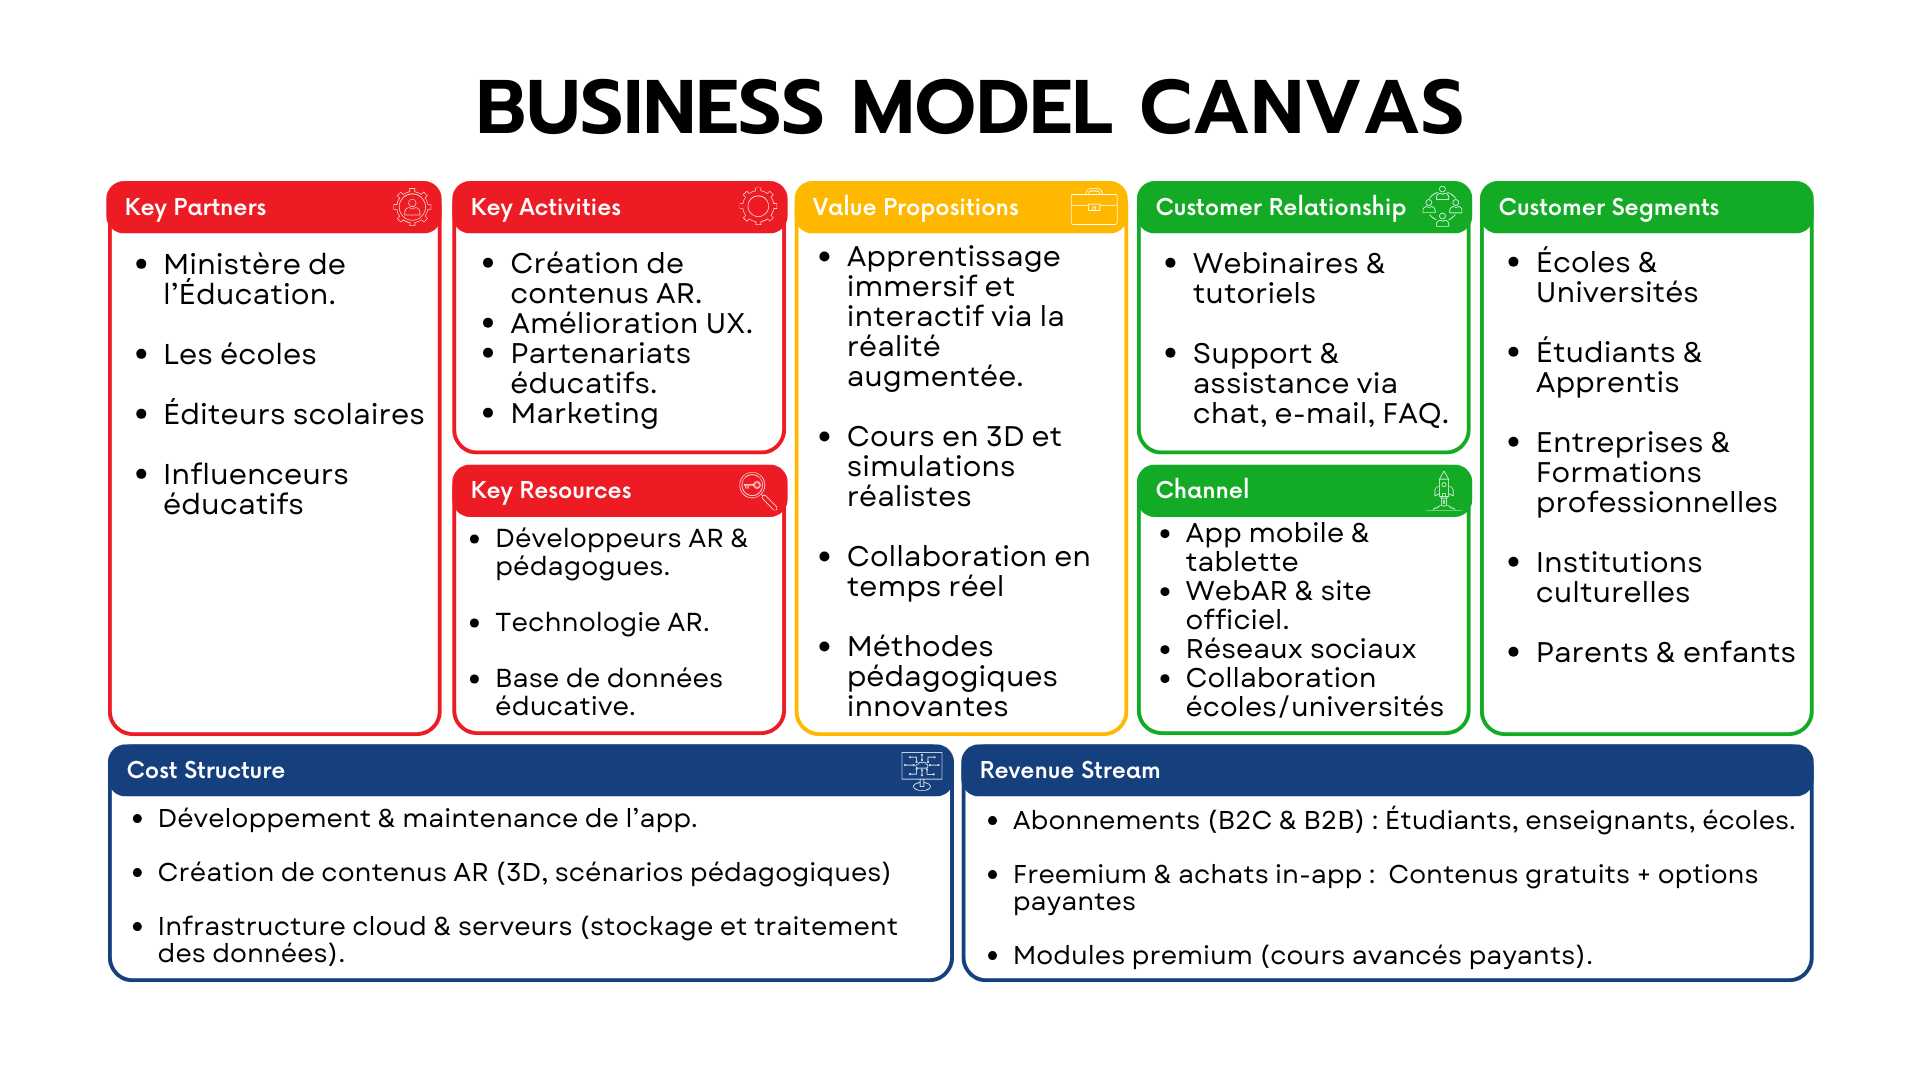
\includegraphics[width=1\textwidth]{images/business_model.png}
	\caption{Business Model}
	\label{fig:sample}
\end{figure}


\chapter{System Design \& Architecture}

\section{Mobile App (Android + AR)}
\begin{itemize}
	\item \textbf{Augmented Reality Framework:}
	\begin{itemize}
		\item \textbf{ARCore:} Google's AR framework for Android, providing powerful and easy-to-integrate AR capabilities.
	\end{itemize}
\end{itemize}

\section{Web Platform (Backend \& Frontend)}
\begin{itemize}
	\item \textbf{Backend:}
	\begin{itemize}
		\item \textbf{Framework:} Spring Boot (Java)
		\item \textbf{Database:} MySQL
		\item \textbf{ORM:} Spring Data JPA/Hibernate
		\item \textbf{File Storage:} Google Cloud Storage (for handling GLB files and other assets)
		\item \textbf{Authentication:} Keycloak (for secure and scalable user authentication)
		\item \textbf{REST APIs:} RESTful API architecture for seamless communication between the frontend, mobile app, and backend services.
	\end{itemize}
	
	\item \textbf{Frontend:}
	\begin{itemize}
		\item \textbf{Framework:} React.js (for building a responsive and dynamic user interface)
	\end{itemize}
\end{itemize}

\section{Cloud Infrastructure \& Deployment}
\begin{itemize}
	\item \textbf{Cloud Provider:} Google Cloud Platform (GCP)
	\begin{itemize}
		\item Scalable and reliable cloud infrastructure for hosting backend services, databases, and file storage.
		\item Integration with ARCore and other Google services for enhanced functionality.
	\end{itemize}
\end{itemize}

\begin{figure}[htbp]
	\centering
	
\includegraphics[width=1\textwidth]{images/system1.png}
	\caption{System Design}
	\label{fig:sample}
\end{figure}

	
	
	
\end{document}